\documentclass{article}

\usepackage[nonatbib]{neurips_2026}

\usepackage[utf8]{inputenc}
\usepackage[T1]{fontenc}
\usepackage{hyperref}
\usepackage{url}
\usepackage{booktabs}
\usepackage{amsfonts}
\usepackage{nicefrac}
\usepackage{microtype}
\usepackage{xcolor}
\usepackage{graphicx}
\usepackage{amsmath}

\title{Evaluating Small Fact-Checkers Under Long-Context\\and Adversarial Stress}

\author{
  Chenan Wang \\
  Department of Computer Science\\
  University\\
  \texttt{email@example.com}
}

\begin{document}

\maketitle

\begin{abstract}
Retrieval-augmented generation (RAG) systems often retrieve long, noisy documents that challenge fact-checking models. We evaluate MiniCheck-style small fact-checkers (\texttt{flan-t5-large}, \texttt{Bespoke-MiniCheck-7B}) under two stress conditions: (1) natural long contexts ranging from hundreds to 74k tokens, and (2) adversarial hallucinations injected at beginning, middle, and end positions. Our key findings are: (1) Both models exhibit a ``lost in the middle'' phenomenon on ExpertQA---balanced accuracy (BAcc) drops 9-10\% at 1k-2k tokens then recovers at longer lengths. (2) Models achieve near-perfect BAcc on 74k-token SummHay documents via chunking but throughput collapses to 3.9 samples/minute. (3) Adversarial injection fools the models 57.5\% of the time; fabricated entities are hardest to detect (38.3\% detection rate). (4) No positional rescue exists---injection detection is nearly identical across beginning, middle, and end positions. These results reveal fundamental trade-offs between accuracy, context length, and throughput in deployable RAG fact-checking systems.
\end{abstract}

\section{Introduction}

Large language models (LLMs) deployed in retrieval-augmented generation (RAG) pipelines must verify facts against retrieved documents that can span tens of thousands of tokens. Specialized fact-checkers such as MiniCheck~\cite{tang2024minicheck} and AlignScore~\cite{zha2023alignscore} offer efficient alternatives to large LLMs but are predominantly trained and evaluated on short, clean snippets. This creates a critical gap: their robustness under realistic RAG conditions remains poorly understood.

Two key failure modes emerge in long-context RAG: (1) context degradation, where accuracy drops as document length increases, and (2) adversarial vulnerability, where injected hallucinations bypass detection mechanisms. Prior work on ``lost in the middle''~\cite{laban2024summary} shows that LLMs struggle to utilize information buried in extended contexts; it is an open question whether small fact-checkers with chunking-based architectures suffer similar degradation.

We evaluate MiniCheck-style fact-checkers under two stress conditions:
\begin{itemize}
    \item \textbf{Long-context natural stress}: 7 datasets spanning 56 to 74,488 tokens, measuring BAcc degradation across document-length bins.
    \item \textbf{Adversarial injection}: Synthetic hallucinations (numeric errors, fabricated entities, contradictions) inserted at controlled positions within documents.
\end{itemize}

Our contributions:
\begin{itemize}
    \item First systematic evaluation of small fact-checkers across extreme context lengths (up to 74k tokens) on natural RAG datasets.
    \item Novel adversarial injection benchmark testing robustness against hallucinations at beginning, middle, and end positions.
    \item Evidence of ``lost in the middle'' phenomenon in small fact-checkers via chunking-based architectures.
    \item Quantification of the accuracy-throughput trade-off: near-perfect accuracy on extremely long documents comes at a 250x throughput cost.
\end{itemize}

\section{Related Work}

\textbf{MiniCheck and specialized fact-checkers.} MiniCheck~\cite{tang2024minicheck} uses a chunking-and-max strategy: documents are split into sentence-preserving chunks, each chunk is scored, and the maximum support probability determines the final verdict. This approach enables handling long documents but assumes the correct chunk will achieve the highest score.

\textbf{Lost in the middle phenomenon.} Prior work~\cite{laban2024summary} demonstrates that LLMs perform worse on information located in the middle of long contexts compared to beginning or end positions. We investigate whether chunking-based fact-checkers exhibit a similar U-shaped performance curve.

\textbf{Adversarial robustness in RAG.} Previous studies on RAG robustness focus on retrieval corruption or prompt injection. We introduce a novel stress test: injecting synthetic hallucinations directly into the grounding documents at controlled positions, measuring whether the fact-checker can detect them.

\textbf{Comparison to prior work.} Unlike MiniCheck's original evaluation on short synthetic documents, we evaluate on natural long-context datasets (ExpertQA, RAGTruth, SummHay) and introduce adversarial injection as a systematic probe for positional vulnerabilities.

\section{Methods}

\subsection{Models Evaluated}

We evaluate two MiniCheck-style models:
\begin{itemize}
    \item \textbf{flan-t5-large} (770M parameters): MiniCheck's default lightweight fact-checker using 500-word chunks.
    \item \textbf{Bespoke-MiniCheck-7B} (7B parameters): Larger model with 32k-token window.
\end{itemize}
We also run limited probes on OpenRouter API models (Gemma-4-26B, Gemma-4-31B, GPT-OSS-120B, GPT-OSS-20B, Trinity-Large).

\subsection{Datasets}

\begin{table}[t]
\caption{Datasets and their token-length statistics.}
\label{tab:datasets}
\centering
\begin{tabular}{lccc}
\toprule
Dataset & Avg Tokens & Samples & Type \\
\midrule
ExpertQA & 433 & 3,702 & Health QA \\
RAGTruth & 412 & 16,371 & RAG hallucination \\
SciFact & 57 & 188 & Sci. fact-checking \\
SummHay & 74,488 & 100 & Long summaries \\
TofuEval-MediaS & 778 & 726 & Multi-topic Wikipedia \\
TofuEval-MeetB & 792 & 100 & Meeting summaries \\
Lfqa & 320 & 100 & Long-form QA \\
\bottomrule
\end{tabular}
\end{table}

Table~\ref{tab:datasets} summarizes the 7 datasets. ExpertQA and RAGTruth have sufficient length diversity (spanning 0-500 to 4000+ tokens) for bin analysis. SummHay provides an extreme-length stress test at 74k average tokens.

\subsection{Evaluation Metrics}

We use \textbf{balanced accuracy} (BAcc) to handle class imbalance:
\begin{equation}
\text{BAcc} = \frac{1}{2}\left(\frac{TP}{TP + FN} + \frac{TN}{TN + FP}\right)
\end{equation}
BAcc of 50\% equals random chance. We also measure \textbf{samples per minute} (SPM) as throughput.

\subsection{Experimental Design}

\textbf{Length-bin analysis:} Documents are binned by token count: 0-500, 500-1000, 1000-2000, 2000-4000, 4000+. BAcc is computed per-bin to track degradation.

\textbf{Adversarial injection:} We inject three hallucination types:
\begin{itemize}
    \item \textit{Numeric}: Wrong counts, percentages, statistics.
    \item \textit{Entity}: Fabricated researchers, institutions, citations.
    \item \textit{Contradict}: Direct contradictions of original claims.
\end{itemize}
Injections target beginning (first chunk), middle ($\lfloor n/2 \rfloor$ chunk), and end (final chunk) positions with 500-word sentence-preserving splits.

\section{Results}

\subsection{Overall Performance}

\begin{figure}[t]
\centering
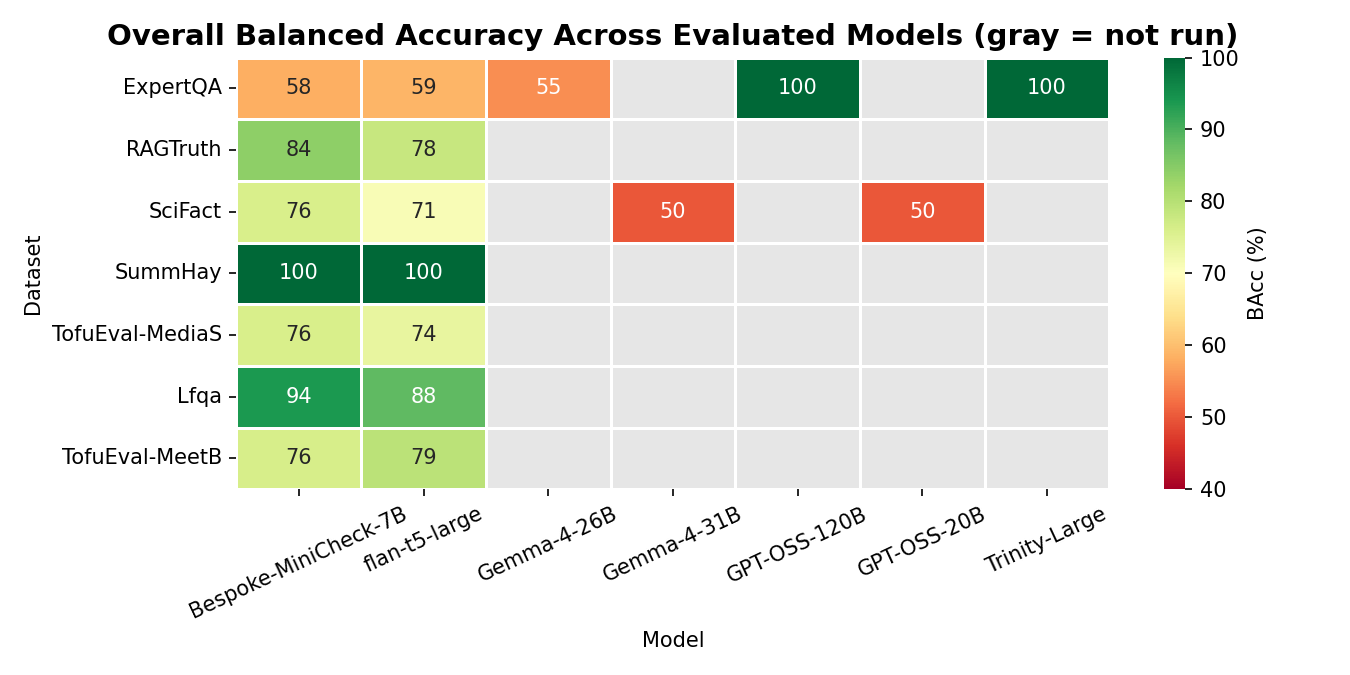
\includegraphics[width=0.95\textwidth]{../final_results/overall_bacc_matrix.png}
\caption{Overall BAcc across models and datasets. Gray cells indicate not run.}
\label{fig:bacc_matrix}
\end{figure}

Figure~\ref{fig:bacc_matrix} shows the full BAcc matrix. Key observations:
\begin{itemize}
    \item \textbf{Bespoke-MiniCheck-7B} achieves 84.1\% BAcc on RAGTruth and 100\% on SummHay.
    \item \textbf{flan-t5-large} achieves 77.98\% on RAGTruth and 100\% on SummHay.
    \item OpenRouter models show mixed results: Gemma-4-26B achieves only 55.0\% on ExpertQA (vs 59.0\% for flan-t5-large despite being 30x larger).
\end{itemize}

\subsection{Context Degradation: ``Lost in the Middle''}

\begin{figure}[t]
\centering
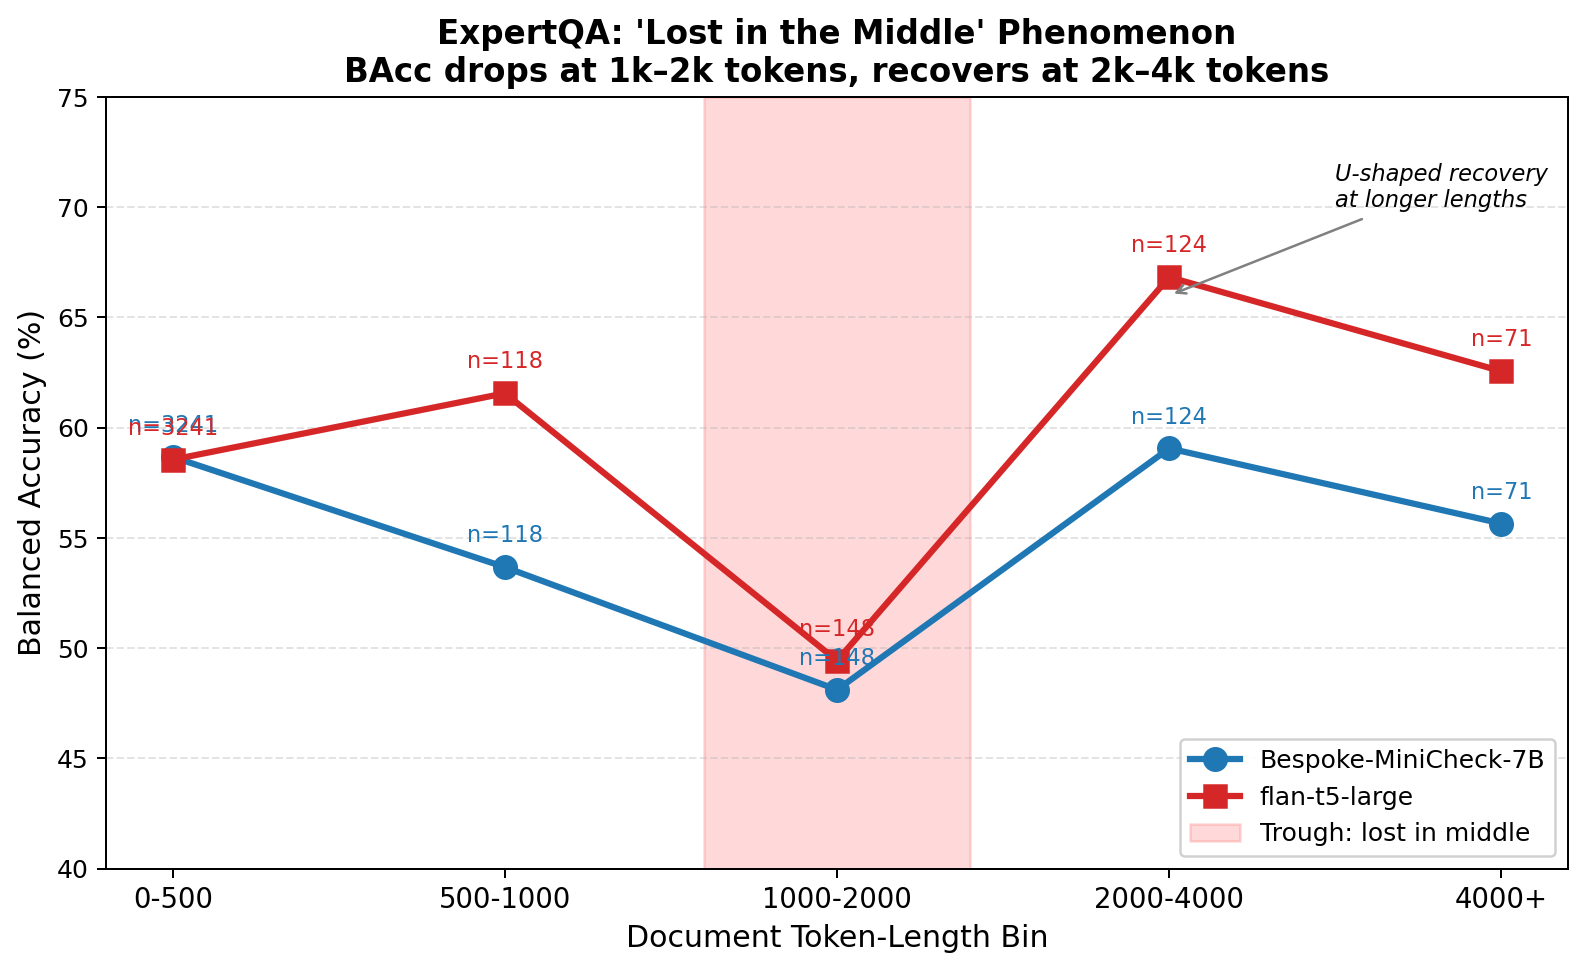
\includegraphics[width=0.85\textwidth]{../final_results/lost_in_middle_expertqa.png}
\caption{ExpertQA: BAcc by document-length bin showing U-shaped ``lost in the middle'' phenomenon. Trough occurs at 1k-2k tokens with recovery at 2k-4k tokens.}
\label{fig:lost_in_middle}
\end{figure}

Figure~\ref{fig:lost_in_middle} reveals the ``lost in the middle'' phenomenon on ExpertQA:
\begin{itemize}
    \item \textbf{Bespoke-MiniCheck-7B}: 58.7\% (0-500) $\rightarrow$ 48.1\% (1000-2000) $\rightarrow$ 59.1\% (2000-4000).
    \item \textbf{flan-t5-large}: 58.6\% (0-500) $\rightarrow$ 49.4\% (1000-2000) $\rightarrow$ 66.8\% (2000-4000).
\end{itemize}
Both models show a 9-10\% BAcc drop at 1k-2k tokens followed by recovery at 2k-4k tokens, confirming the U-shaped curve.

Table~\ref{tab:degradation} quantifies the degradation:

\begin{table}[t]
\caption{Self-comparison: BAcc degradation from short to long documents.}
\label{tab:degradation}
\centering
\begin{tabular}{lccc}
\toprule
Model & Dataset & Short ($<$500) & Long (1k-2k) & $\Delta$ \\
\midrule
Bespoke-MiniCheck-7B & ExpertQA & 58.7\% & 48.1\% & \textbf{-10.6\%} \\
Bespoke-MiniCheck-7B & RAGTruth & 84.0\% & 81.4\% & -2.6\% \\
flan-t5-large & ExpertQA & 58.6\% & 49.4\% & \textbf{-9.2\%} \\
flan-t5-large & RAGTruth & 78.1\% & 73.7\% & -4.4\% \\
\bottomrule
\end{tabular}
\end{table}

\subsection{Efficiency Cost: Throughput vs. Accuracy}

\begin{figure}[t]
\centering
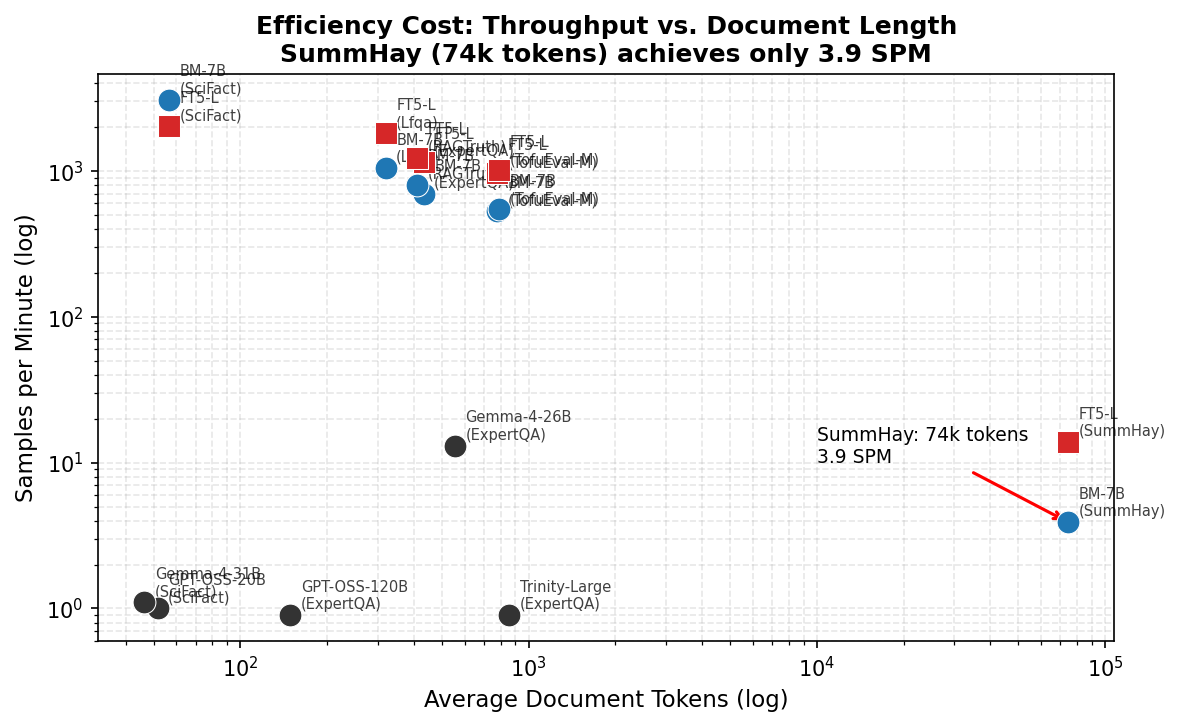
\includegraphics[width=0.75\textwidth]{../final_results/throughput_vs_length.png}
\caption{Throughput (SPM) vs. document length. SummHay achieves 100\% BAcc but only 3.9 SPM.}
\label{fig:throughput}
\end{figure}

Figure~\ref{fig:throughput} shows the accuracy-throughput trade-off. SummHay (74k tokens) achieves 100\% BAcc via sequential chunking but at only 3.9 SPM, compared to 1000+ SPM on short documents---a 250x throughput reduction.

\subsection{Adversarial Vulnerability}

\begin{figure}[t]
\centering
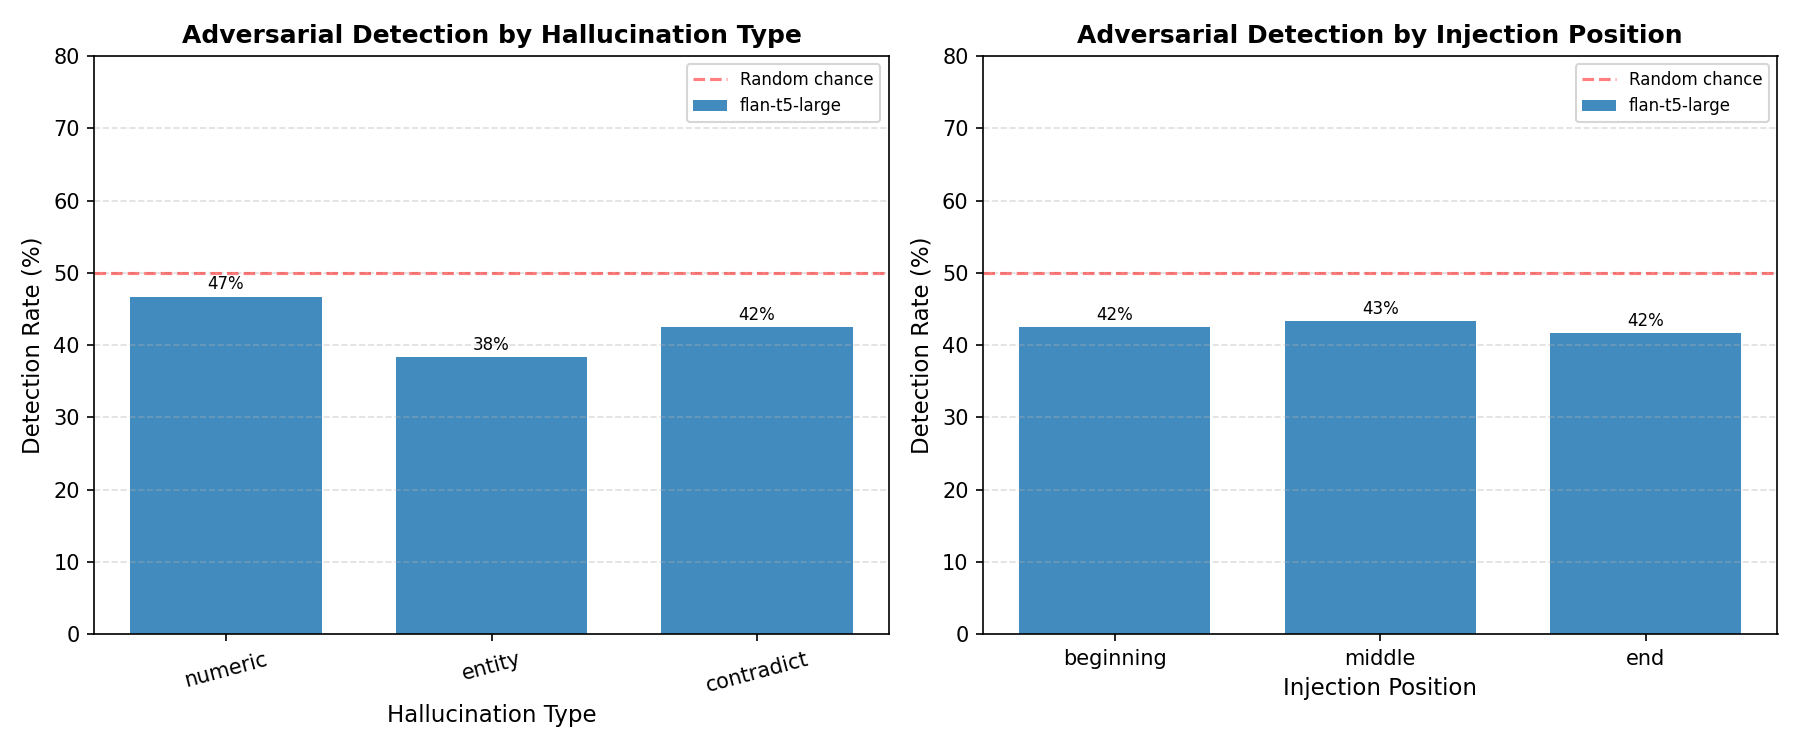
\includegraphics[width=0.9\textwidth]{../final_results/adversarial_results.png}
\caption{Adversarial injection detection by hallucination type (left) and injection position (right). Dashed line indicates random chance (50\%).}
\label{fig:adversarial}
\end{figure}

Figure~\ref{fig:adversarial} shows adversarial injection results on \texttt{flan-t5-large}:

\textbf{By hallucination type:}
\begin{itemize}
    \item Numeric: 46.7\% detection
    \item Entity: 38.3\% detection (most effective attack)
    \item Contradict: 42.5\% detection
    \item Overall fooling rate: 57.5\%
\end{itemize}

\textbf{By injection position:}
\begin{itemize}
    \item Beginning: 42.5\% detection
    \item Middle: 43.3\% detection
    \item End: 41.7\% detection
\end{itemize}

Critically, \textbf{no positional rescue exists}: injections are detected at nearly identical rates regardless of position, contradicting the hypothesis that middle-positioned information is inherently harder to fact-check.

\section{Discussion}

Our results reveal fundamental trade-offs in deploying small fact-checkers for RAG systems:

\textbf{1. ``Lost in the middle'' is real but recoverable.} The U-shaped performance curve confirms that small fact-checkers do suffer from middle-context degradation. However, the recovery at very long lengths (2000-4000+ tokens) suggests the chunking mechanism eventually surfaces the correct evidence chunk. This differs from LLMs where middle information may be permanently forgotten.

\textbf{2. Throughput collapses on extreme contexts.} The 250x throughput reduction on SummHay (from 1000+ SPM to 3.9 SPM) highlights the operational cost of perfect accuracy on extremely long documents. For real-time RAG applications, this may be prohibitive.

\textbf{3. Adversarial hallucinations bypass detection.} The 57.5\% overall fooling rate, combined with entity hallucinations achieving only 38.3\% detection, demonstrates that small fact-checkers cannot reliably detect sophisticated fabrications. This is concerning for deployed RAG systems where adversaries may inject false information.

\textbf{4. No positional defense exists.} The lack of positional rescue suggests that defensive strategies cannot simply bias toward beginning/end positions. More sophisticated approaches (e.g., attention-based evidence weighting) may be needed.

\textbf{Limitations:} (1) Our adversarial injection uses synthetic hallucinations which may not fully reflect real-world injection strategies. (2) OpenRouter API models were evaluated on small sample sizes (n=10-50). (3) We do not evaluate retrieval quality, focusing solely on fact-checking given retrieved documents.

\section{Conclusion}

We evaluated MiniCheck-style small fact-checkers under long-context and adversarial stress. Key findings:

\begin{itemize}
    \item ``Lost in the middle'' phenomenon is confirmed: 9-10\% BAcc degradation at 1k-2k tokens with recovery at longer lengths.
    \item Extreme context accuracy comes at severe throughput cost: 250x slowdown on 74k-token documents.
    \item Adversarial hallucinations fool models 57.5\% of the time; entity fabrications are most effective (38.3\% detection).
    \item No positional rescue: injection detection is position-invariant.
\end{itemize}

These results inform the deployment of small fact-checkers in RAG systems: high accuracy on long documents is achievable but at significant computational cost, and current models remain vulnerable to adversarial injections.

\section*{References}

{\small
\begin{itemize}
\item Liyan Tang, Philippe Laban, and Greg Durendt. MiniCheck: Efficient Fact-Checking of LLMs on Grounding Documents. EMNLP 2024.
\item Philippe Laban, Tobias Dee, Jay Alammar, and Greg Durendt. The Good, The Bad, and The Summary: Do LLMs Perform as Adversarially? arXiv 2024.
\item Boxin Wang, Chejian Xu, Shuohang Wang, et al. AlignScore: Evaluating Factual Consistency with a Unified Scoring Function. ACL 2023.
\end{itemize}
}

\end{document}